% FinMesh paper: IEEE conference format (IEEEtran). DRAFT for the authors to edit.
% Figures and tables are generated by `uv run finmesh paper-assets` from the committed
% result pages; regenerate them rather than editing them by hand. Every number in the text
% comes from those pages (docs/eval/test, docs/eval/a25, docs/gates).
% Build: pdflatex main && bibtex main && pdflatex main && pdflatex main
% (use the official IEEEtran.cls / IEEEtran.bst of your venue's template, e.g. Overleaf's).
\documentclass[conference]{IEEEtran}
\IEEEoverridecommandlockouts
\usepackage{cite}
\usepackage{amsmath,amssymb}
\usepackage{graphicx}
\usepackage{array}
\usepackage{pifont}
\usepackage{url}
\newcommand{\cmark}{\ding{51}}
\newcommand{\xmark}{\ding{55}}
\graphicspath{{figures/}}

\begin{document}

\title{Minimised Evidence Sharing for Cross-Bank Money-Laundering Detection:\\
Pre-Registered Sealed Tests and Fresh Replication on AMLworld}

\author{\IEEEauthorblockN{Allaudin Ansari}
\IEEEauthorblockA{\textit{Affiliation} \\ City, Country \\ email}
\and
\IEEEauthorblockN{Ravi}
\IEEEauthorblockA{\textit{Affiliation} \\ City, Country \\ email}}

\maketitle

\begin{abstract}
Money-laundering schemes are spread across banks, so each bank's monitoring sees only a
fragment and rarely links the parts. We study a protocol in which banks exchange
\emph{minimised evidence} about counterparties---a calibrated score bucket and bucketed
behaviour counters, keyed by pseudonymous tokens from an oblivious pseudorandom
function---and evaluate it under a discipline uncommon in this area: every hypothesis is
pre-registered, decided once on a sealed test, and then confirmed on two further test
windows that were never opened during development. On AMLworld, sharing raises linked
scheme detection from 0.063 to 0.534 on the high-illicit fresh test (gain 0.47, 95\% CI
[0.43, 0.51]) and recovers 0.92 of the gain of a pooled relational oracle; the gain holds on
all four sealed tests, without suspected dataset artefacts, and on a base detector that
outperforms published gradient-boosting results on the standard benchmark. Analysts
review 6.8--8.5$\times$ fewer alerts per linked scheme. A leakage audit with explicit attacks
finds that a bare alert flag reveals high fan-in in the low-illicit regime; a gated flag,
chosen on validation by a frozen rule, removes the leak on fresh data at no detection cost.
We report the claims that failed---typology attribution and the token re-identification
target---alongside those that held.
\end{abstract}

\begin{IEEEkeywords}
anti-money laundering, inter-bank information sharing, privacy-enhancing technologies,
oblivious pseudorandom functions, pre-registration, leakage audit
\end{IEEEkeywords}

% =========================================================================================
\section{Introduction}

Laundering schemes deliberately cross institutional boundaries: funds are gathered at one
bank, layered through accounts at others and paid out elsewhere. Each bank's transaction
monitoring sees only the legs that touch its own customers. The result is a familiar
pattern in practice---many isolated alerts, few connected cases---and a familiar question:
how much would banks gain by sharing what they know, and what would sharing reveal?

Prior work answers the first half with federated learning, secure computation or
supervisory analytics (Section~\ref{sec:related}), usually on one data split chosen and
reported by the same team, and answers the second half by the properties of a mechanism
rather than by measuring what a curious peer can infer. We take a different route on both.

\emph{Evidence, not models.} When a bank's detector flags an account, it can ask the banks
that hold the account's counterparties for a minimised evidence record about them: a score
bucket and bucketed behaviour counters, keyed by a token that only an online, metered,
logged service can produce. A ladder of sharing levels (S0--S4, plus progressive
disclosure) separates what each extra field buys from what it reveals.

\emph{Evaluation as a sealed test.} Hypotheses, metrics, operating points and model
settings were registered at the outset; provisional thresholds were fixed once, from
validation, at a pre-planned gate, and everything was frozen before the test was
opened~\cite{nosek2018}. Each frozen configuration was evaluated once on a sealed test, with
every opening logged. Improvements
made after that test were developed on validation data only, frozen by written selection
rules, and confirmed on two further 16-day windows of AMLworld~\cite{altman2023} that had
never been opened.

\emph{Contributions.}
\begin{itemize}
\item A minimised evidence-sharing protocol for cross-bank detection, with OPRF
tokens~\cite{rfc9497}, a fusion layer and a pooled linking rule, and a ladder of sharing
levels that isolates the value of each disclosure.
\item A pre-registered evaluation on four sealed tests, two of them fresh: sharing raises
linked scheme detection by 0.38--0.57 over local monitoring and recovers 0.64--0.98 of a
pooled relational oracle's gain; the gain survives removing suspected artefact features and
replacing the detector with one that outperforms published gradient-boosting baselines.
\item An empirical leakage audit that found, and a pre-registered fix that closed, an
attribute leak through alert flags.
\item Case-quality measures that matter to investigators: more complete cases and
6.8--8.5$\times$ fewer alerts per linked scheme.
\item A negative result on narrative generation with small local language models, and a
select-then-template design that is grounded by construction.
\end{itemize}

% =========================================================================================
\section{Related Work}\label{sec:related}

\emph{Collaborative detection.} Federated learning lets banks exchange model updates
instead of data: Suzumura et al.~\cite{suzumura2019} proposed federated graph learning across
banks, and Zheng et al.~\cite{zheng2025} train a federated graph network on country-level
subgraphs of AMLworld. The US/UK PETs Prize financial-crime track produced systems that bring
a bank's private account flags into a payment hub's model: with MPC and federated
learning~\cite{arora2023}, private set intersection and secure aggregation~\cite{abadi2024starlit},
or differential privacy with secure summation~\cite{khan2024fedrd}. Secure computation has
been used to propagate risk scores across banks~\cite{vanegmond2024} and to trace money flows
at national scale under homomorphic encryption~\cite{brand2023fintracer}; Project
Aurora~\cite{bis2023aurora} compared siloed, national and cross-border collaborative analysis
on synthetic payments.

\emph{What differs.} Table~\ref{tab:related} compares these works. We share evidence about
counterparties rather than models, and we measure leakage with explicit attacks instead of
relying on a mechanism's guarantee alone. None of the works above reports results on a
pre-registered, sealed test, and several select models on the split they report; none
replicates on data never opened during development.

\emph{Benchmarks.} AMLworld~\cite{altman2023} provides synthetic transactions with laundering
labels and typologies. Multigraph GNNs~\cite{egressy2024} and subgraph features with gradient
boosting~\cite{blanusa2024} set the transaction-level state of the art; we anchor our detector
against those published numbers.

\begin{table*}[!t]
\centering
\caption{Collaborative anti-money-laundering and financial-crime detection: what is shared, how it is protected, and how it is evaluated}
\label{tab:related}
\footnotesize
\setlength{\tabcolsep}{3pt}
\begin{tabular}{*{6}{>{\raggedright\arraybackslash}p{2.55cm}}}
\hline
Work & Shared between institutions & Protection & Data & Evaluation & Privacy evidence \\
\hline
Suzumura et al.\ \cite{suzumura2019} & Model parameters (global graph features planned) & Federated learning; DP/MPC proposed, not evaluated & Simulated, six banks (FCA TechSprint) & One test split, prototype & None \\
Arora et al.\ \cite{arora2023} & Bank account flags, inside a payment hub's training & Federated learning + MPC (oblivious transfer, secret sharing), noise & PETs Prize synthetic payments & Challenge test environment & Design argument \\
Abadi et al.\ \cite{abadi2024starlit} & Identity alignment and model updates & Private set intersection + secure federated learning & Synthetic payments & Scalability and accuracy, prototype & Security proof \\
Khan et al.\ \cite{khan2024fedrd} & Embeddings and gradients & Differential privacy + secure summation & PETs Prize synthetic, AMLSim & One test split; best test epoch reported & Formal DP bound \\
van Egmond et al.\ \cite{vanegmond2024} & Encrypted risk scores, propagated across banks & Secure multi-party computation & One bank's transactions & Precision at fixed recall & Design argument \\
Brand et al.\ \cite{brand2023fintracer} & Encrypted flow-tracing indicators & Homomorphic encryption & Nation-scale deployment & Run time only & Design argument \\
BIS Innovation Hub \cite{bis2023aurora} & Collaborative analysis and learning & Privacy-enhancing technologies & Synthetic, national and cross-border & Scenario comparison & Not reported \\
Zheng et al.\ \cite{zheng2025} & Model updates and aggregated node embeddings & Federated learning (no formal guarantee) & AMLworld HI-Small subset \cite{altman2023} & One split (5\% train) & None \\
\hline
This work & Minimised evidence records keyed by OPRF tokens; alert flags, gated & Pseudonymous tokens (OPRF), data minimisation, flag gating; LDP and progressive disclosure as options & AMLworld HI/LI Medium and two never-opened Large windows \cite{altman2023} & Pre-registered sealed tests, fresh replication, 95\% CIs, Holm & Empirical attacks (4 targets) and token re-identification \\
\hline
\end{tabular}
\end{table*}


% =========================================================================================
\section{System}\label{sec:system}

\subsection{Setting and threat model}
A federation of banks each sees the transactions with one end at its own customers,
including the counterparty's account and bank, and nothing more. Adversaries are
honest-but-curious: a peer bank follows the protocol but inspects every token, request and
response it receives, and holds candidate account lists from its own payments; the token
service sees blinded queries and does not collude with banks. Poisoning, collusion and
compromised hosts are out of scope. No legal or regulatory claim is made.

\subsection{Local detection (S0)}
Each bank scores every active account in every 6-hour window with a LightGBM
model~\cite{ke2017lightgbm} on 47 features in four families (behaviour, graph, history,
neighbourhood), each computed from the current window and the previous 72 hours of the
bank's own view. Scores are calibrated per bank, and each bank alerts a fixed number of
account-windows per window (Section~\ref{sec:method}), so sharing cannot raise recall by
raising alert volume. A bank links its own alerts into incidents when the accounts
transacted directly within 72 hours.

\subsection{Tokens}
Banks must recognise that the account a peer asks about is one they paid, without exchanging
account numbers and without holding a key that tokenises arbitrary identifiers. Each bank
blinds an identifier and sends it to a token service, which evaluates a pseudorandom function
under a per-epoch key (one epoch is seven days) without seeing the identifier, following the
OPRF construction of RFC~9497~\cite{rfc9497}. Tokenising a candidate therefore needs an
online, logged query, and each bank has a per-epoch budget, sized to twice the largest
legitimate use on validation. Shared-key hashing is kept only as a positive control in the
audit.

\subsection{Evidence and sharing levels}
An account-window above the evidence floor (calibrated probability $\geq 0.01$) or alerted
asks, for each counterparty at another bank within the 72-hour lookback, what that bank
holds. The responding bank answers according to the sharing level:
\begin{itemize}
\item \textbf{S1}: whether it has alerted the counterparty (alert flag), with a time bucket.
\item \textbf{S2}: a minimised record---probability bucket; up to three deviating features
with direction and a coarse magnitude; bucketed fan-in, fan-out and pass-through, and
cross-bank, new-counterparty and amount counters. No raw values.
\item \textbf{S3}: S2 with every field except the time bucket and flag released through
$k$-ary randomised response~\cite{warner1965,dwork2006} at a total $\varepsilon\in\{0.5,
\dots, 8\}$ per record, capped per account and epoch.
\item \textbf{S4}: S2 plus an 8-dimensional autoencoder embedding (a leakage upper reference).
\item \textbf{PD}: progressive disclosure---the S1 answer, plus the S2 record only when the
requester's own score bucket is at least $\tau\in\{2,3,4\}$.
\item \textbf{Gated flag} (S1F, added in Section~\ref{sec:a25}): the S1 flag is returned only
when the requester's score bucket is at least 2.
\end{itemize}

\subsection{Fusion and linking}
Each bank combines its own score with the returned evidence (counts of requests, flags and
records; the highest and summed probability buckets; fan and pass-through buckets) in a
per-bank logistic stacker, cross-fitted on the two halves of validation. Banks then cut their
own queues at the same alert budget, and alerts are linked across banks when their accounts
transacted within 72 hours (the pooled linking rule). Two pooled references bound the
ladder: the \emph{oracle}, one LightGBM on every bank's data, and the \emph{relational oracle},
which adds to each pooled score its counterparties' pooled scores across the whole
federation. The relational oracle is the ceiling in all ratios below.

\subsection{Case narratives}
A gradient-boosted attributor assigns a typology to each linked case from the fused evidence
(or leaves it unattributed below a confidence threshold). A local language model then writes
a short narrative under a JSON schema whose typology must equal the attributed one and whose
cited fields must exist in the evidence; failed checks trigger one retry, then a fixed
template. The select-then-template variant (N4) asks the model only to choose up to four
evidence fields; fixed templates write every sentence.

% =========================================================================================
\section{Evaluation Method}\label{sec:method}

\subsection{Data and federation}
We use the IBM AMLworld synthetic data~\cite{altman2023} in its high-illicit (HI) and
low-illicit (LI) variants. Table~\ref{tab:datasets} lists the four sealed tests. For each set,
a label-free rule finds the dense period of transactions and keeps 16 days (Medium: the whole
dense period; Large: the last 16 days of its dense period). Windows are 6 hours; train,
validation and test take 60/20/20\% of the windows, with a one-window gap at each boundary.
All banks are grouped into eight institutions balanced by accounts (federation B8), so every
account is held by a member.

\begin{table}[!t]
\centering
\caption{Test sets}
\label{tab:datasets}
\footnotesize
\setlength{\tabcolsep}{4pt}
\begin{tabular}{lrrrr}
\hline
Test set & Transactions & Laundering & Schemes & Cross-member \\
 & (millions) & rows & & test schemes \\
\hline
HI-Medium & 31.9 & 31,146 & 2,756 & 480 \\
LI-Medium & 31.3 & 15,270 & 456 & 91 \\
HI-Large & 30.3 & 39,798 & 6,638 & 559 \\
LI-Large & 29.7 & 18,037 & 896 & 78 \\
\hline
\end{tabular}
\par\smallskip\parbox{\linewidth}{\scriptsize Each set is a 16-day dense window of AMLworld, split by 6-h window 60/20/20 into train, validation and test with one-window gaps; eight institutions (federation B8) hold every account. Cross-member test schemes: laundering schemes in the test partition that touch two or more institutions. Medium: the primary tests; Large: the replication tests.}
\end{table}


\subsection{Unit, labels and metrics}
The unit is the account-window: an account held at a member in one window with at least one
transaction. It is positive if it touches a laundering leg of a scheme assigned to its own
partition; legs of schemes assigned to another partition, and busy accounts that a scheme
crossed once (at least 20 legs, under 10\% laundering), are masked. Each bank alerts one
account per 1,000 accounts per day, exactly. A scheme is \emph{detected} if any of its
account-windows is alerted within 72 hours of its first window, and \emph{linked}---the
primary metric---if at least two of its accounts fall in one incident within that time.
Before any sharing level was built, a gate required the oracle to beat S0 by at least 0.05 in
linked detection on validation: it did by 0.508 [0.465, 0.550] on HI-Medium, almost entirely
through linking (any-alert detection: S0 0.864, oracle 0.886).

\subsection{Pre-registration and the sealed test}
Hypotheses (Table~\ref{tab:results}), operating points, model settings and statistical rules
were registered at the outset. Thresholds marked provisional could be revised once, from
validation, at a pre-planned gate (G1), after which the pre-registration was frozen; model
settings were never tuned on validation. Every later change is an amendment logged with its
reason and date, made before the results it affects existed. Test labels are held behind a seal. Every configuration is scored on test without
labels; a SHA-256 digest of the scores is logged with the single opening allowed per
experiment, dataset and seed. A repeat is allowed only after a crash, and is logged. The
week-18 tests (HI- and LI-Medium) decided the pre-registered hypotheses.

\subsection{Fresh replication (amendment A25)}\label{sec:a25}
Improvements made after the week-18 test could not be scored on that test without tuning on
it. They were therefore developed on Medium validation only and selected by rules written
before the candidates ran:
\begin{itemize}
\item \emph{Protected flag}: among randomised-response and gated variants of the S1 flag,
the one within the privacy margin on every target of both Medium sets with the largest share
of the plain flag's gain. This selected the gated flag, with 1.01 of the gain.
\item \emph{Narrative}: among four local models (3--8 B parameters), the highest strict
grounding; N4 built on it if at least as grounded. This selected N4 on \texttt{qwen3:8b}.
\item \emph{Benchmark adequacy}: if our pooled detector fell more than 5 F1 points below
published LightGBM results on the benchmark's validation split, add a stronger detector as an
extra track. It fell 14.5 points below on HI-Medium, so a transaction-level detector
(Section~\ref{sec:robust}) was added (S0+, S2+, oracle+).
\end{itemize}
The owner then signed a frozen commit, and the two Large windows were opened once per
experiment and seed: the main track, an artefact-free track and the stronger-detector track.

\subsection{Statistics}
Headline configurations ran with five seeds and the others with three; a seed fixes model
training and negative sampling. Per-scheme outcomes are averaged over seeds before a
cluster bootstrap over schemes (1,000 replicates). Gains are paired over the same schemes,
with Holm correction~\cite{holm1979} across the eleven sharing configurations compared with
S0.

\subsection{Leakage audit}
A curious peer attacks everything it receives (seed 0 of each run). A1 re-identifies tokens
from candidate lists of its own counterparties, under hashing and under the OPRF budget. A2
infers whether the queried account transacted with a third member; A3 infers top-decile
outgoing amount, top-decile fan-in and pass-through behaviour. The A2/A3 attacker is a
gradient-boosted classifier trained on the true attributes of half the queried accounts;
the baseline is a prior-only classifier on what the peer knew before asking. The
pre-registered margin requires the upper 95\% bound of (attack $-$ prior) true-positive rate
at 1\% false-positive rate to be at most 0.05 on every target, for S1 and for S3 at
$\varepsilon\leq2$.

% =========================================================================================
\section{Results}\label{sec:results}

\subsection{Detection}
Fig.~\ref{fig:ladder} and Table~\ref{tab:results} summarise the sealed tests. Local
monitoring links few schemes: 0.063--0.136 of them. Minimised evidence (S2) raises linked
detection to 0.702 (HI-Medium) and 0.657 (LI-Medium) on the week-18 tests, and to 0.534
(HI-Large) and 0.450 (LI-Large) on the fresh tests; every gain has its 95\% interval above
zero after Holm correction, and random alerts at the same budget link none. S2 recovers 0.98,
0.79, 0.92 and 0.64 of the relational oracle's gain, meeting the pre-registered 0.60 on all
four tests, although the LI-Large interval reaches 0.52. Most of the value arrives with the
alert flag alone (S1: 0.516 on HI-Large), as the gate result suggested: the gap is in linking
alerts across banks, not in detecting them. Plain pooling is not the ceiling: one model on
every bank's data, linked by the same rule, reaches 0.434 on HI-Large, below S2.

\begin{figure}[!t]
\centering
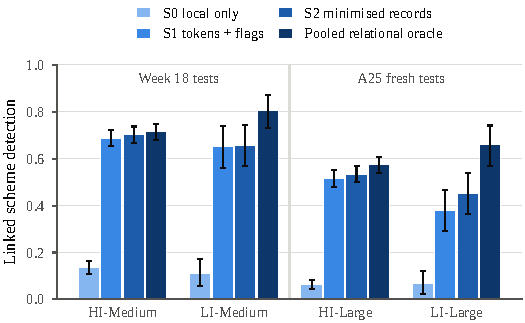
\includegraphics[width=\columnwidth]{fig_ladder}
\caption{Linked scheme detection on the four sealed tests by sharing level: local only
(S0), tokens and alert flags (S1), minimised evidence records (S2), and a pooled
relational oracle that sees every bank's data. Bars: mean over seeds; whiskers: 95\% scheme
bootstrap intervals. HI- and LI-Medium were decided on the week-18 tests; HI- and LI-Large
are the A25 windows, never opened during development.}
\label{fig:ladder}
\end{figure}

\begin{table*}[!t]
\centering
\caption{Pre-registered claims on the sealed tests}
\label{tab:results}
\footnotesize
\setlength{\tabcolsep}{4pt}
\begin{tabular}{lcccc}
\hline
Pre-registered claim & HI-Medium & LI-Medium & HI-Large & LI-Large \\
\hline
H1a: S2 $-$ S0 linked detection & 0.57 [0.53, 0.61] \cmark & 0.55 [0.45, 0.63] \cmark & 0.47 [0.43, 0.51] \cmark & 0.38 [0.29, 0.48] \cmark \\
H1b: share of oracle gain ($\geq$0.60) & 0.98 [0.94, 1.03] \cmark & 0.79 [0.69, 0.88] \cmark & 0.92 [0.87, 0.97] \cmark & 0.64 [0.52, 0.77] \cmark \\
H1c: plain flag, fan-in advantage & $-$0.002 [$-$0.008, 0.003] \cmark & 0.092 [0.079, 0.103] \xmark & 0.001 [$-$0.002, 0.003] \cmark & 0.043 [0.031, 0.059] \xmark \\
\quad gated flag (A25) & --- & --- & 0.001 [$-$0.001, 0.003] \cmark & 0.004 [0.000, 0.007] \cmark \\
H1d: PD gain share, least disclosure & 0.98 at 0.07 \cmark & 0.99 at 0.01 \cmark & 0.95 at 0.03 \cmark & 0.81 at $<$0.01 \cmark \\
H3a: attribution above baselines & \cmark & \xmark & \xmark & \xmark \\
H3b: narrative grounding ($\geq$0.95) & 0.86 [0.81, 0.90] \xmark & 0.92 [0.84, 0.96] \xmark & 1.00 [0.98, 1.00] \cmark & 0.95 [0.87, 0.98] \cmark \\
PT2: hashing $\div$ OPRF re-id. ($\geq$10) & 19.9 \cmark & 8.7 \xmark & 8.1 \xmark & 9.3 \xmark \\
\hline
\end{tabular}
\par\smallskip\parbox{\linewidth}{\scriptsize Sealed tests; 95\% intervals from a scheme bootstrap. H1c: upper 95\% bound of (attack $-$ prior) TPR at 1\% FPR at most 0.05 on every attack target (A2, A3); the value shown is the binding target, A3 fan-in, and the mark is the verdict over all targets and, for the plain flag, the S3 levels with $\varepsilon\leq 2$. H1d: PD configuration reaching $\geq$0.80 of S2's gain with the smallest share of S2's disclosed accounts. H3b on Medium: free-text narratives (A23); on Large: select-then-template (N4). Medium columns: week-18 tests; Large: A25 fresh tests.}
\end{table*}


\subsection{Robustness}\label{sec:robust}
\emph{Artefacts.} The two strongest features in every model are AMLworld payment-format
shares and self-transfers, which may be simulator quirks. Without them (Fig.~\ref{fig:robustness}),
the gain is 0.438 on HI-Large and 0.210 on LI-Large, both with intervals above zero. On
LI-Large the alert flag alone then carries little (S1 0.054) while the records keep 0.217: the
minimised record, not the flag, carries the signal there.

\emph{A stronger detector.} On AMLworld's published split, a transaction-level LightGBM on
the transaction's own fields and both accounts' features (Table~\ref{tab:benchmark})
outperforms both published gradient-boosting baselines on all four sets and the best
published GNN on two. Used as the local detector (S0+), it leaves the sharing gain in place:
0.433 on HI-Large and 0.355 on LI-Large. Its pooled version, however, is much stronger on
LI-Large (0.764), so S2+ recovers only 0.49 of the corresponding relational oracle's gain
there---the one robustness rule that missed.

\begin{figure}[!t]
\centering
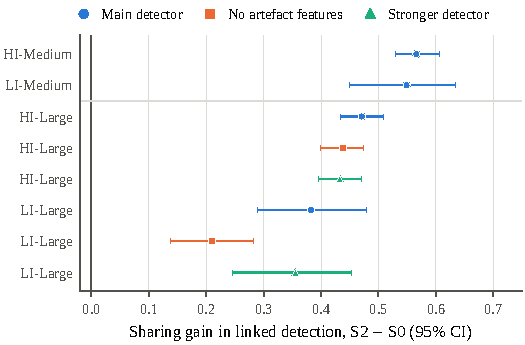
\includegraphics[width=\columnwidth]{fig_robustness}
\caption{Sharing gain (S2 $-$ S0 linked detection) with 95\% intervals. Main detector on
all four tests; on the Large tests also without the suspected artefact features
(payment-format shares, self-transfers) and with a stronger transaction-level detector
that outperforms both published gradient-boosting baselines on the AMLworld benchmark
(Table~\ref{tab:benchmark}).}
\label{fig:robustness}
\end{figure}

\begin{table}[!t]
\centering
\caption{Detector against published results}
\label{tab:benchmark}
\footnotesize
\setlength{\tabcolsep}{4pt}
\begin{tabular}{lcc}
\hline
Model & HI-Medium & LI-Medium \\
\hline
Ours, account-window detector & 42.67 $\pm$ 2.76 & 24.08 $\pm$ 2.01 \\
Ours, transaction model & 67.01 $\pm$ 2.27 & 34.34 $\pm$ 1.55 \\
LightGBM + GFP \cite{egressy2024} & 59.48 & 20.85 \\
XGBoost + GFP \cite{egressy2024} & 65.70 & 28.16 \\
Multi-PNA + EU \cite{egressy2024} & 66.48 & 36.07 \\
\hline
\end{tabular}
\par\smallskip\parbox{\linewidth}{\scriptsize Minority-class F1 (\%) on AMLworld's published split (all transactions, by day 60/20/20), threshold chosen on validation; ours: mean $\pm$ s.d. over 5 seeds. Pooled data in every row (the published models see all banks).}
\end{table}


\subsection{Privacy}
\emph{Attribute leakage.} On the high-illicit tests the alert flag and the LDP records stay
within the margin. On the low-illicit tests they do not (Fig.~\ref{fig:privacy}): a peer
that receives flags infers top-decile fan-in with an advantage of 0.092 on LI-Medium and 0.043
[0.031, 0.059] on LI-Large, because in that regime an alert is itself informative about an
account's in-degree. S3 does not help, since it does not perturb the flag. The gated flag,
selected on validation, brings the advantage to 0.004 [0.000, 0.007] on LI-Large and keeps
1.00 (HI) and 0.93 (LI) of the plain flag's detection gain. Records (S2, S4) disclose
attributes by design: the fan-in advantage is 0.73--0.74.

\emph{Progressive disclosure.} PD at $\tau=4$ keeps 0.95 (HI-Large) and 0.81 (LI-Large) of
S2's gain while disclosing records on 3\% and under 1\% as many accounts. On the
high-illicit sets this is uninformative, because the flag alone already reaches 0.95 of S2.

\emph{Tokens.} Under hashing, a peer re-identifies 0.39 of other banks' record tokens on
HI-Large; under the OPRF budget, 0.049. The ratio (8.1 on HI-Large, 9.3 on LI-Large, 8.7 on
LI-Medium, 19.9 on HI-Medium) misses the pre-registered factor of 10 on three of four tests.
Legitimate token use stayed within the frozen budget on both fresh tests. An adaptive budget
(twice the previous epoch's use), replayed on recorded use, kept refusals far above its 1\%
target on busy days and lowered the ratio to 2.6--3.2 even under honest use; it was not
adopted.

\begin{figure}[!t]
\centering
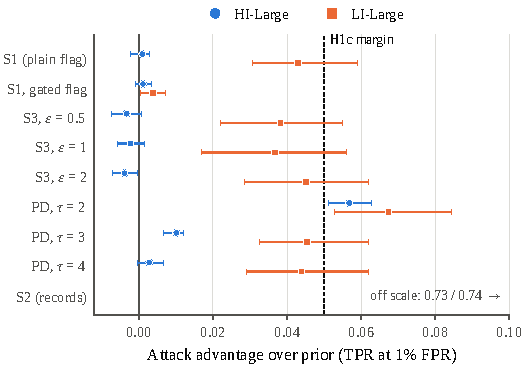
\includegraphics[width=\columnwidth]{fig_privacy}
\caption{Leakage audit on the Large tests: advantage of a strong attacker over a prior-only
attacker in inferring whether a queried account has top-decile fan-in (the binding target),
true-positive rate at 1\% false-positive rate, with 95\% intervals. The dashed line is the
pre-registered margin (upper bound $\leq$ 0.05). On LI-Large the plain alert flag and every
level that carries it exceed the margin; the gated flag chosen on validation does not.}
\label{fig:privacy}
\end{figure}

\subsection{Case quality and analyst workload}
For an investigator, a linked case should contain the scheme and nothing else. With
sharing, the largest case holds 0.77 of a scheme's accounts on HI-Large, against 0.47 locally,
and a scheme is split into 1.05 cases instead of 1.51 (Table~\ref{tab:casequality}). Because
every bank keeps the same alert budget, the cost per linked scheme falls sharply: 18 alerts
instead of 153 on HI-Large and 140 instead of 944 on LI-Large (Fig.~\ref{fig:workload}).

\begin{figure}[!t]
\centering
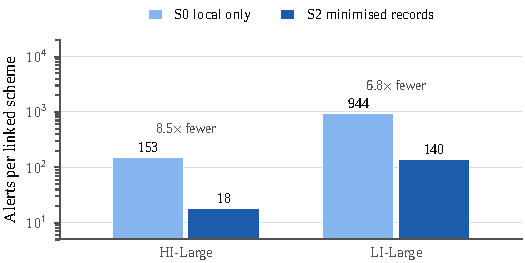
\includegraphics[width=\columnwidth]{fig_workload}
\caption{Alerts an analyst reviews per laundering scheme linked, local-only monitoring (S0)
versus minimised evidence sharing (S2), on the Large tests (logarithmic axis).}
\label{fig:workload}
\end{figure}

\begin{table}[!t]
\centering
\caption{Case quality and analyst workload}
\label{tab:casequality}
\footnotesize
\setlength{\tabcolsep}{4pt}
\begin{tabular}{lrrrr}
\hline
Measure & \multicolumn{2}{c}{HI-Large} & \multicolumn{2}{c}{LI-Large} \\
 & S0 & S2 & S0 & S2 \\
\hline
Scheme accounts in the case & 0.47 & 0.77 & 0.48 & 0.73 \\
Cases per linked scheme & 1.51 & 1.05 & 1.49 & 1.06 \\
Alerts per linked scheme & 153 & 18 & 944 & 140 \\
\hline
\end{tabular}
\par\smallskip\parbox{\linewidth}{\scriptsize Per detected scheme, seed-averaged: share of the scheme's accounts in its largest case (completeness), number of cases it is split into (fragmentation), and alerts raised per scheme linked (analyst workload). Replication tests, seeds 0--4.}
\end{table}


\subsection{Attribution and narratives}
Typology attribution from fused evidence beat local attribution and both baselines on
HI-Medium but not on LI-Medium or either fresh test; we treat it as exploratory. Free-text
narratives from small local models were grounded in their structure---valid JSON, the right
typology, existing fields---in 0.86 (HI-Medium) and 0.92 (LI-Medium) of first replies, short
of the 0.95 target. Larger models (7--8 B) did not fix this: strict grounding, which also
requires correct numbers, scope and claims, stayed at 0.06--0.22 on validation
(Table~\ref{tab:narrative}). Select-then-template (N4) met the target on both fresh tests
(1.00 and 0.95), and an automated judge rated its validation texts faithful in all 30 sampled
cases, against 21--29 for free text.

\begin{table}[!t]
\centering
\caption{Case narratives: local models and select-then-template}
\label{tab:narrative}
\footnotesize
\setlength{\tabcolsep}{4pt}
\begin{tabular}{lccc}
\hline
Design & Grounding & Strict & Faithful \\
\hline
\multicolumn{4}{l}{\emph{HI-Medium validation, 200 cases (judge: 30)}} \\
N0: \texttt{llama3.2:3b}, free text & 0.96 & 0.13 & 21/30 \\
N1: \texttt{qwen2.5:7b}, free text & 0.97 & 0.10 & 26/30 \\
N2: \texttt{llama3.1:8b}, free text & 0.99 & 0.06 & 29/30 \\
N3: \texttt{qwen3:8b}, free text & 0.98 & 0.22 & 23/30 \\
N4: select-then-template (N3) & 0.99 & 0.83 & 30/30 \\
\hline
\multicolumn{4}{l}{\emph{N4 on the replication tests}} \\
HI-Large & 1.00 & 0.82 & --- \\
LI-Large & 0.95 & 0.56 & --- \\
\hline
\end{tabular}
\par\smallskip\parbox{\linewidth}{\scriptsize Grounding (H3b): first reply is valid, keeps the attributed typology and cites only evidence fields. Strict: also 1--4 fields, every number from the evidence, claim consistency and scope. Faithful: automated judge (one rater, not blind) on the 30-case sheet; delivered text after retry and template fallback.}
\end{table}


% =========================================================================================
\section{Limitations}
AMLworld is synthetic; the results show what minimised sharing can achieve on the field's
standard benchmark, not on real bank data. The low-illicit windows are small (78--91
cross-member test schemes), so their intervals are wide. The audit covers honest-but-curious
peers and four attribute targets; collusion, poisoning and side channels are out of scope,
and S1, S2 and PD responses are minimised and audited but not differentially private. The
narrative judge is a single automated rater, neither blind nor independent of the template
design. A federated, differentially private neural scorer, also pre-registered, met its target on
LI-Medium but not on HI-Medium, where a strong local detector left little for it to add.
Finally, every amendment after the pre-registration is logged with its reason. Two changed how
token requests are metered so that runs would not stop on a token cap (A24a, A25a), both before
the tests they affected were opened; one fixed a report page after an opening without changing
any score (A24b).

% =========================================================================================
\section{Conclusion}
Sharing a little evidence about counterparties---a flag and a bucketed record, keyed by
metered tokens---lets banks link several times more laundering schemes than local
monitoring, close to what pooling all data would achieve, at a fraction of the alerts. The
result held on four sealed tests, two of them never opened during development, without
suspected artefacts and on a competitive base detector. Measuring leakage with attacks, rather
than asserting it, found a real leak in the simplest disclosure and a fix that held on fresh
data. We hope the evaluation discipline---pre-registration, sealed tests, logged openings and
fresh replication---proves as useful to collaborative financial-crime research as the
protocol itself.

\section*{Data and code availability}
AMLworld is available under CDLA-Permissive-2.0. Code, the pre-registration, every amendment,
the sealed-test access log and the result pages are in the project repository (MIT licence);
every figure and table is regenerated by one command from the committed result pages.

\bibliographystyle{IEEEtran}
\bibliography{references}

\end{document}
